\documentclass{article}
\usepackage{booktabs}
\usepackage[pdftex]{graphicx}
\usepackage[T1]{fontenc}
\usepackage[margin=1in]{geometry}
\DeclareGraphicsRule{*}{mps}{*}{}

\title{An App Store}
\author{William Deprez}
\date{May 17, 2019}

\begin{document}
%\maketitle
\begin{titlepage}
    \centering
    {\scshape\LARGE Plano East Senior High School \par}
    \vspace{1cm}
    {\scshape\Large Final database project\par}
    \vspace{1.5cm}
    {\huge\bfseries An App Store\par}
    \vspace{2cm}
    \Large\textit{William Deprez}
    \vfill
    {\large May 17, 2019\par}
\end{titlepage}

\section{Introduction}
My program will implement a database of Users, Apps, and Reviews to make up a social app store.
It tracks a user’s owned apps, existing apps, and reviews of that app.
This creates a useful store and essentially it’s own digital marketplace where anyone can create their own applications.
My list of apps will be contained within a store object, while my users are contained within my community object.

\section{Application Architecture}

The application contains several components which are depicted in Figure~\ref{UML}.
I will use three plain java objects for my program.
My first object App will contain the name of the app, the creator (username), the appId, and the date of creation.
The second object User will contain the username, userId, ownedApps, and usersReviews.
The third object Review will store a rating --- an integer of one through ten --- and some review related text.
\begin{figure}[h]
    \centering
    \includegraphics[height=6.1in]{uml.1}
    \caption{UML Architecture Diagram\label{UML}}
\end{figure}

\section{Application Views}
See Figure~\ref{views} for application view.
The application will have the following pages:
\begin{itemize}
    \item{Login Splash}
    \item{Main Menu}
    \item{Community}
    \item{Store}
\end{itemize}
\begin{figure}[ht!]
    \centering
    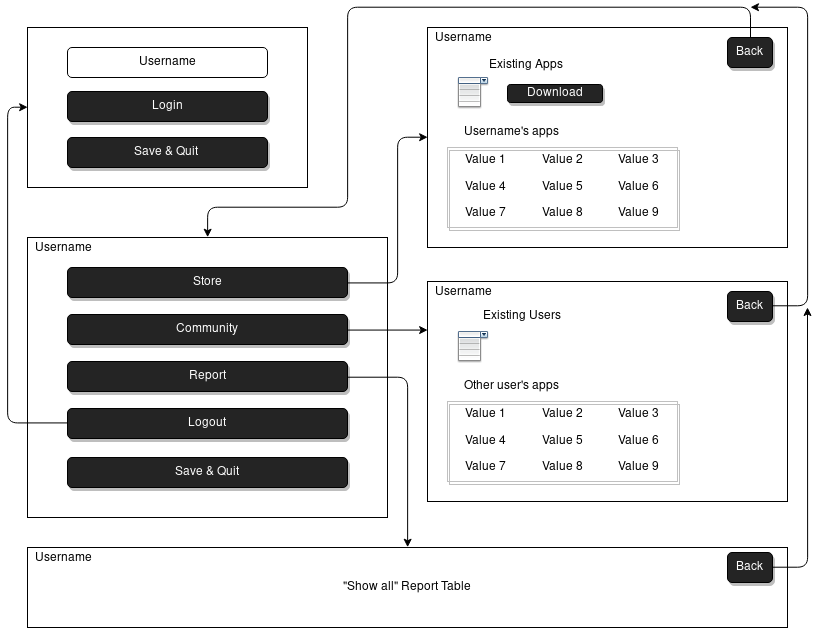
\includegraphics[width=.85\textwidth]{views.png}
    \caption{Views Diagram\label{views}}
\end{figure}
\subsection{Login Splash}
The login splash page will have a username field and a login button.
Additionally this page will have a quit button.
\subsection{Main Menu}
The main menu view will have the following buttons:
\begin{itemize}
    \item{Store}
        --- Clicking this button will change the view to the store view.
    \item{Community}
        --- Clicking this button will change the view to the community view.
    \item{Report}
        --- Clicking this button will open a dialogue box with the report view.
    \item{Logout}
        --- Clicking this button will return the view to the login splash view.
    \item{Save \& Quit}
        --- Clicking this button will store all data in the SQLite database and exit the application.
\end{itemize}
\subsection{Store}
The store view allows the current user to add or remove apps from their inventory.
This view will also provide a list of the current inventory.

\noindent{The store view consists of the following components:}
\begin{itemize}
    \item{Label}
        --- name of current user.
    \item{Combo box}
        --- contains available apps.
    \item{App add button}
        --- adds the currently selected item in combo box to inventory if not already therein.
    \item{Inventory list box}
        --- contains a list of current apps associated with the current user.
    \item{Delete selected app button}
    \item{Make review button}
        --- opens option pane with the following:
        \begin{itemize}
            \item{Combo box}
            \item{Save review button}
        \end{itemize}
    \item{Back button}
        --- returns to main menu view.
\end{itemize}

\subsection{Community}
This view will also a user to view the apps owned other users and the potential reviews of those apps.
\begin{itemize}
    \item{Label}
        --- name of current user.
    \item{Combo box}
        --- contains list of all other users.
    \item{App inventory list box}
        --- contains a list of the selected user's apps.
    \item{Back button}
        --- returns to main menu view.
\end{itemize}

\subsection{Report}
Table~\ref{table:user-showall} contains an example ``show all'' report of the apps owned by each user.
Table~\ref{table:app-showall} contains an example ``show all'' report of the apps owned by each user.
The report view will have two sections showing (1) the apps owned by each user, and (2) the users that own each app.

\begin{table}[ht!]
    \centering
    \noindent\begin{tabular}{*{5}{c}}
        \toprule
        userId & userName & appId & appName & review \\
        \midrule
        1 & ``Amelia47'' & 1 & ``Flappy Bird'' & ``This game is so addicting\ldots guh!'' \\
        1 & ``Amelia47'' & 5 & ``Chess'' & null \\
        1 & ``Amelia47'' & 23 & ``Angry Birds'' & ``Old but gold!'' \\
        4 & ``William123'' & 3 & ``Battleship'' & null \\
        5 & ``Ashley'' & 3 & ``Battleship'' & null \\
        5 & ``Ashley'' & 5 & ``Chess'' & ``Way too hard!'' \\
        \bottomrule
    \end{tabular}
    \caption{User database information\label{table:user-showall}}
\end{table}

\begin{table}[ht!]
    \centering
    \noindent\begin{tabular}{*{5}{c}}
        \toprule
        appId & appName & userId & userName & review \\
        \midrule
        1 & ``Flappy Bird'' & 1 & ``Amelia47'' & ``This game is so addicting\ldots guh!'' \\
        3 & ``Battleship'' & 4 & ``William123'' & null \\
        3 & ``Battleship'' & 5 & ``Ashley'' & null \\
        5 & ``Chess'' & 1 & ``Amelia47 & null \\
        5 & ``Chess'' & 5 & ``Ashley'' & ``Way too hard!'' \\
        23 & ``Angry Birds'' & 1 & ``Amelia47'' & ``Old but gold!'' \\
        \bottomrule
    \end{tabular}
    \caption{App database information\label{table:app-showall}}
\end{table}

\section{Class Descriptions}
\subsection{Driver}
\subsubsection{Description}
The Driver class creates an object of itself for JFrame. Additionally, it creates an instance of Community, Store, and Database. It passes the data from the database to the Community and Store on startup.
\subsubsection{Methods}
\begin{itemize}
    \item{public static void main(String[] args)}
        --- The main method for the project.
    \item{private Driver()}
        --- Creates an instance of a JFrame inside of main
\end{itemize}
\subsection{Database}
\subsubsection{Data}
The class will only store a String that contains the url of the database.
\subsubsection{Methods}
\begin{itemize}
    \item{public Database()}
        --- creates a database object.
    \item{public void connect()}
        --- connects to the database.
    \item{public void createUserTable()}
        --- creates the user table.
    \item{public void dropUserTable()}
        --- drops the user table from the database.
    \item{public void saveUsers(List<User> users)}
        --- overwrites the existing table with the new arraylist.
    \item{public List<User> loadUsers()}
        --- returns the user table as an arraylist.
    \item{public void createAppTable()}
        --- creates the app table.
    \item{public void dropAppTable()}
        --- drops the app table from the database.
    \item{public void saveApps(List<App> apps)}
        --- overwrites the existing table with the new arraylist.
    \item{public List<App> loadApps()}
        --- returns the app table as an arraylist.
\end{itemize}
\subsection{Community}
\subsubsection{Data}
The Community class' sole instance field contains a list of User objects
\subsubsection{Methods}
\begin{itemize}
    \item{public Community(List<User> users)}
        --- creates a community object.
    \item{public List<User> getUsers()}
        --- returns an arraylist of users, primarily for use in conjunction with the 'saveApps()' method of the database class.
    \item{public void setUsers(List<User> users)}
        --- replaces the existing class attribute `users'.
    \item{public void addUser(User user)}
        --- adds a user to the community list.
    \item{public void sort()}
        --- sorts the list using a merge sort.
    \item{public boolean hasUser(String userName)}
        --- returns a boolean for if the username was found within the `users' list.
    \item{public User getUser(String userName)}
        --- returns the `User' object which matches contains the implicit parameter `userName' which matches the parameter.
    \item{public void removeUser(String userName)}
        --- removes the `User' object which username matches.
    \item{public String toString()}
        --- returns the data as a String
\end{itemize}
\subsection{Store}
\subsubsection{Data}
Stashes a list of `App' objects.
\subsubsection{Methods}
\begin{itemize}
    \item{public Store(List<App> apps)}
        --- creates a Store object
    \item{public List<App> getUsers()}
        --- returns the arraylist of apps
    \item{public void setApps(List<App> apps)}
        --- replaces `apps' with passed list.
    \item{public void addApp(App app)}
        --- adds an app object to the end of the list.
    \item{public void sort()}
        --- sorts the list using a merge sort.
    \item{public boolean hasApp(String appName)}
        --- returns a boolean for if the appName is found within the `apps' list
    \item{public User getApp(String appName)}
        --- returns the `App' with the matching appName.
    \item{public void removeApp(String appName)}
        --- removes `App' with matching appName.
    \item{public String toString()}
        --- returns the list of apps as a String.
\end{itemize}
\subsection{User}
\subsubsection{Data}
\begin{itemize}
    \item{int userId}
        --- the userId used for sorting within the database.
    \item{String userName}
        --- the userName of the `User' object.
    \item{List<Integer> userApps}
        --- the list of apps the user owns.
\end{itemize}
\subsubsection{Methods}
\begin{itemize}
    \item{public User(int userId, String userName)}
        --- creates a `User' object, with a userId based on size of `users' list within community and a userName based on the users input passed from main.
    \item{public int getUserId()}
        --- returns the userId of the `User' object.
    \item{public void setUserId(int userId)}
        --- replaces the userId with parameter.
    \item{public int getUserName()}
        --- returns the username of the `User' object.
    \item{public void setUserName(String userName)}
        --- replaces the implicit userName with the parameter.
    \item{public List<Integer> getUserApps()}
        --- returns the `userApps' list
    \item{public void setUserApps(List<Integer> userApps)}
        --- replaces the existing userApps list with the parameter.
    \item{public void addUserApp(int userId)}
        --- adds the userId to the `userApps' list.
    \item{public boolean isUserApp(int appId)}
        --- returns true if appId is found within `userApps'.
    \item{public void removeUserApp(int appId)}
        --- removes appId from `userApps' list.
    \item{public int compareTo(Object other)}
        --- returns the difference of the implicit userId by other's userId.
    \item{public boolean equals(Object other)}
        --- returns true if userId and userName Strings match.
    \item{public String toString()}
        --- returns the `User' object as a String, containing its instance fields.
\end{itemize}
\subsection{App}
\subsubsection{Data}
\begin{itemize}
    \item{int appId}
        --- the appId used for sorting within the database.
    \item{String appName}
        --- the appName of the `App' object.
    \item{List<Integer> appOwners}
        --- the userIds of the `User' objects that own the `App' object.
\end{itemize}
\subsubsection{Methods}
\begin{itemize}
    \item{public App(int appId, String appName, int creatorId)}
        --- creates an `App' object.
    \item{public void int getAppId()}
        --- returns the implicit appId.
    \item{public void setAppId(int appId)}
        --- sets the implicit appId to the parameter.
    \item{public String getAppName()}
        --- returns the implicit appName.
    \item{public void setAppName(String appName)}
        --- sets the implicit appName to the parameter.
    \item{public List<Integer> getAppOwners()}
        --- returns the `appOwners'.
    \item{public void setAppOwners(List<Integer> appOwners)}
        --- sets the implicit `appOwners' to the parameter.
    \item{public void addAppOwner(int appId)}
        --- adds the appId to the `appOwners' list.
    \item{public boolean isAppOwner(int userId)}
        --- returns true if userId is found within `appOwners'.
    \item{public void removeAppOwner(int userId)}
        --- removes userId from `appOwners' list if isAppOwner(userId) returns true.
    \item{public int compareTo(Object other)}
        --- returns the difference of the implicit appId by other's appId.
    \item{public boolean equals(Object other)}
        --- returns true if appId matches.
    \item{public String toString()}
        --- Returns the object as a String.
\end{itemize}

\section{Application Storage}
The storage for this application will be SQLite.
The following tables are required for basic functionality:
\begin{itemize}
    \item{user\_tb}
        --- stores the userId and userName for the community.
    \item{app\_tb}
        --- stores the appId, appName, and the creator's userId for the store.
    \item{userapp\_tb}
        --- stores the relationship between each appId and userId along with an optional review.
\end{itemize}
The tables used within the database are depicted in Table~\ref{table:user_tb}, Table~\ref{table:app_tb}, and Table~\ref{table:userapp_tb} below.
%The user\_tb will store all the userId and userName for the community.
%The app\_tb will store all the appId, appName, and the creator's userId for the store.
%The userapp\_tb junction will store the relationship between each appId and userId along with an optional review.

\begin{table}[ht!]
    \centering
    \noindent\begin{tabular}{*{2}{c}}
        \toprule
        userId (int, primary key, \& autoincrement) & userName (varchar (32), not null, \& unique)\\
        \midrule
        1 & ``Amelia47'' \\
        2 & ``1John'' \\
        3 & ``Samantha99'' \\
        4 & ``William123'' \\
        5 & ``Ashley'' \\
        \bottomrule
    \end{tabular}
    \caption{the user\_tb table of the program's SQLite database\label{table:user_tb}}
\end{table}
\begin{table}[ht!]
    \centering
    \noindent\begin{tabular}{*{3}{c}}
        \toprule
        appId (int, primary key, \& autoincrement) & appName (varchar (64), not null, \& unique) & creatorId (int)\\
        \midrule
        1 & ``Flappy Bird'' & 3 \\
        2 & ``Chess'' & 5 \\
        3 & ``Battleship'' & 23 \\
        4 & ``Learn Languages'' & 4 \\
        \bottomrule
    \end{tabular}
    \caption{the app\_tb table of the program's SQLite database\label{table:app_tb}}
\end{table}
\begin{table}[ht!]
    \centering
    \noindent\begin{tabular}{*{3}{c}}
        \toprule
        appId (int) & userId (int) & review (varchar (2000))\\
        \midrule
        23 & 1 & ``I like this game!'' \\
        1101 & 43 & null\\
        50 & 2643 & null\\
        23 & 2 & ``This game was alright\ldots'' \\
        4 & 703 & null\\
        2 & 4 & ``I love this game'' \\
        \bottomrule
    \end{tabular}
    \caption{the userapp\_tb table of the program's SQLite database\label{table:userapp_tb}}
\end{table}
\end{document}
